
\documentclass[11pt]{article}
\usepackage{verbatim}
\usepackage{listings}
\usepackage{graphicx}
\usepackage{a4wide}
\usepackage{color}
\usepackage{amsmath}
\usepackage{amssymb}
\usepackage[dvips]{epsfig}
\usepackage[T1]{fontenc}
\usepackage{cite} % [2,3,4] --> [2--4]
\usepackage{shadow}
\usepackage{hyperref}
\usepackage{physics}
\usepackage{url}
\usepackage{tikz}
\usepackage{subcaption}


\usetikzlibrary{arrows, shapes}

\setcounter{tocdepth}{2}

\lstset{language=c++}
\lstset{alsolanguage=[90]Fortran}
\lstset{basicstyle=\small}
\lstset{backgroundcolor=\color{white}}
\lstset{frame=single}
\lstset{stringstyle=\ttfamily}
\lstset{keywordstyle=\color{red}\bfseries}
\lstset{commentstyle=\itshape\color{blue}}
\lstset{showspaces=false}
\lstset{showstringspaces=false}
\lstset{showtabs=false}
\lstset{breaklines}

\title{ Project 1 \\ Molecular Dynamics \\ FYS-4460 }
\author{Gullik Vetvik Killie }

\begin{document}

\maketitle

\tableofcontents

\section{Part 1:}
	\subsection{Task a: Creating a FCC lattice}
	This task is implemented in the function createFCCLattice()
	\\ \\
		\noindent The noble gas argon should have a stable lattice structure when a solid, by letting the system start in a stable situation we avoid a lot of energy to be infused into the systems temperature due to it minimizing potential energy. The implementation is done by going through several nodes, \(R_i\), put on a grid in the box and then placing 4 atoms around each node. Let \(c_l\) be the length between nodes.

		\begin{align*}
		\vb{R}_{ij} = \vb{R}_i + \vb{r}_j \qquad{j }= \{1,2,3,4\} \qquad{i = }\{1,2, ... , 4\text{N}_{\text{atoms}}\}
		\end{align*}

		\begin{align*}
			\vb{r}_1 &= 0 \vu{i} + 0 \vu{j} + 0 \vu{k}
			\\
			\vb{r}_2 &= \frac{c_l}{2} \vu{i} + \frac{c_l}{2} \vu{j} + 0 \vu{k}
			\\
			\vb{r}_3 &= 0 \vu{i} + \frac{c_l}{2} \vu{j} + \frac{c_l}{2} \vu{k}
			\\
			\vb{r}_4 &= \frac{c_l}{2} \vu{i} + 0 \vu{j} + \frac{c_l}{2} \vu{k}
		\end{align*}

	\subsection{Task b: Gaussian Velocities}

		\begin{figure}
			\center
			\includegraphics[width = 0.7\textwidth]{Figures/velocityDistributions}
			\caption{The velocites given to the atoms with a gaussian overlay}
		\end{figure}

\subsection{Task e: Computing forces}

\label{sub:potential}

		We will be using the Lennard-Jones potential to approximate the forces between the molecules, which work quite well, given it's simplicity, for neutral particles, especially noble gases, as we are dealing with in this study \cite{Wiki}. The formula is given below.

		\[
		U(r_{ij}) = 4 \epsilon \left[ \left( \frac{\sigma}{r_{ij}} \right)^{12} - \left( \frac{\sigma}{r_{ij}} \right)^{6} \right]
		\]


		
		At short distances the term to the twelfth power dominates and represents a repulsive force, Paulie exclusion principle, while at longer distances the term to sixth power dominates and represents the attractive van der Waal force. The \(\sigma \) is the distance at which the potential is \(0\), while \( \epsilon  \) is the depth of the well. 
		\(\sigma = 3.405 \text{\AA}\) and \(\varepsilon/k_B = 119.8 \text{K}\) are chosen to fit the physical properties of the system for Argon.


		\noindent The force felt between the molecules is given by the negative gradient of the potential.

		\begin{align*} 
		\vb{F}(r_{ij}) &= -\grad U(r_{ij})
		\intertext{The potential only has a nonzero derivative along \( \vb{r}_{ij} \), the  axis between then particles, so it is natural to evaluate the gradient in that coordinate system before projecting it onto the xyz coordinates used by the program.}
		\\
		\vb{F} (r_{ij}) &= - 4 \epsilon  \partial_{r_{ij}}  \left[ \left( \frac{\sigma}{r_{ij}} \right)^{12} - \left( \frac{\sigma}{r_{ij}} \right)^{6} \right] \vu{r}_{ij}
		\\
		\vb{F} (r_{ij}) &= - 4 \epsilon   \left[ -\frac{12}{r_{ij}} \left(  \frac{\sigma}{r_{ij}} \right)^{12} + \frac{6}{r_{ij}} \left( \frac{\sigma}{r_{ij}} \right)^{6} \right] \vu{r}_{ij}
		\\
		\vb{F} (r_{ij}) &= 24 \epsilon   \left[ 2 \left(  \frac{\sigma}{r_{ij}} \right)^{12} - \left( \frac{\sigma}{r_{ij}} \right)^{6} \right] \frac{\vb{r}_{ij}}{r_{ij}^2}
		\\
		m_i\pdv[2]{r_i}{t} &= \sum_j{24 \epsilon   \left[ 2 \left(  \frac{\sigma}{r_{ij}} \right)^{12} - \left( \frac{\sigma}{r_{ij}} \right)^{6} \right] \frac{\vb{r}_{ij}}{r_{ij}^2}}
		\end{align*}

	\subsection{f: NonDimensionality}	
	Now we introduce some new units to get a nondimensional equation of motion. 
		\(
		\begin{cases}
		r & \rightarrow   \sigma r'
		\\
		t & \rightarrow \tau t'
		\end{cases}
		\)

		\begin{align*}
		m_i\pdv[2]{\sigma r'_i}{(\tau t') }  &= \sum_j{24 \epsilon   \left[ 2 \left(  \frac{\sigma}{\sigma r'_{ij}} \right)^{12} - \left( \frac{\sigma}{\sigma r'_{ij}} \right)^{6} \right] \frac{\sigma\vb{r'}_{ij}}{\sigma^2r'^2_{ij}}}
		\\
		\pdv[2]{ r'_i}{(t')} &= \frac{24 \epsilon \tau ^2}{m_i \sigma^2}  \sum_j{  \left[ 2 \left(  \frac{\sigma}{\sigma r'_{ij}} \right)^{12} - \left( \frac{\sigma}{\sigma r'_{ij}} \right)^{6} \right] 
		\frac{\vb{r'}_{ij}}{r_{ij}'^2}}
		\intertext{Choosing \(\tau = \sigma \sqrt{ m/\varepsilon } \) then gives the dimensionless equation}
		\pdv[2]{ r'_i}{(t')} &= 24   \sum_j{  \left[ 2 r'^{-12}_{ij}  - r'^{-6}_{ij} \right] r_{ij}'^{-2}	\vb{r}'_{ij}  }
		\end{align*}



	\subsubsection{Algorithm to implement force}
		The implementation of the force will be along the following steps:
		\begin{itemize}
		\item Find vector between the two particles \( \vb{r}_{ij} = \vb{r}'_i - \vb{r}_j \)
		\item Calculate \(r_{ij}'^2\), \( r_{ij}'^6 \) and \(r_{ij}'^{12}\) for a particle pair
		\item Calculate the modified force \( 24   \sum_j{  \left[ 2 r'^{-12}_{ij}  - r'^{-6}_{ij} \right] r_{ij}'^{-2}  \vb{r}'_{ij}  } \)
		\item Add the force to both particles force account, halves the necessary computations. One positive one negative
		\end{itemize}

\subsection{h: Neighbour lists}
	A simple system of \(3\cross 3\) neighbors, see figure \ref{fig:neighbor_grid} will have all the properties and connections of a larger system, since a neighbor is only connected to the neighbors bordering it. Let us choose the neighbor in the center, \(111\),  and find the neighbors we must go through to find to let it interact with each of it's neighbors once. First we let it interact with the top layer, \ref{fig:top}, and then we note that it is not necessary to let it interact with the bottom layer, since all the cells in that layer will interact with the choosen cell, \(111\). Then we fill the remainer of the front, 

	\tikzstyle{vertex}=[circle,fill=black!25,minimum size=20pt,inner sep=0pt]

	\begin{figure}
		\begin{subfigure}{1\textwidth}
			\begin{subfigure}[b]{0.18\textwidth}
			\begin{tikzpicture}[scale=1.0, auto,swap]
	    		\foreach \pos/\name in {{(2,0)/200}, 	{(2,1)/201},	{(2,2)/202},
	                            		{(1,0)/000}, 	{(1,1)/101}, 	{(1,2)/102},
	                            		{(0,0)/000}, 	{(0,1)/001},	{(0,2)/002}}
	        	\node[vertex] (\name) at \pos {$\name$};
	        \end{tikzpicture}
	        \caption*{j \(= 0\)}
	        \end{subfigure}
	        \qquad \qquad
	        \begin{subfigure}[b]{0.18\textwidth}
			\begin{tikzpicture}[scale=1.0, auto,swap]
	    		\foreach \pos/\name in {{(2,0)/210}, 	{(2,1)/211},	{(2,2)/212},
	                            		{(1,0)/010}, 	{(1,1)/111}, 	{(1,2)/112},
	                            		{(0,0)/010}, 	{(0,1)/011},	{(0,2)/012}}
	        	\node[vertex] (\name) at \pos {$\name$};
	        \end{tikzpicture}
	        \caption*{j \(= 1\)}
	        \end{subfigure}
	        \qquad \qquad
	        \begin{subfigure}[b]{0.18\textwidth}
			\begin{tikzpicture}[scale=1.0, auto,swap]
	    		\foreach \pos/\name in {{(2,0)/220}, 	{(2,1)/221},	{(2,2)/222},
	                            		{(1,0)/020}, 	{(1,1)/121}, 	{(1,2)/122},
	                            		{(0,0)/020}, 	{(0,1)/021},	{(0,2)/022}}
	        	\node[vertex] (\name) at \pos {$\name$};
	        \end{tikzpicture}
	        \caption*{j \(= 2\)}
	        \end{subfigure}
	       	\caption{All the neighbors in a \(3\cross 3\) system divided up into three slices with j constant. The numbers are position in an ijk-grid.}
	       	\label{fig:neighbor_grid}
		\end{subfigure}
		\begin{subfigure}{1\textwidth}
			\begin{subfigure}[b]{0.18\textwidth}
			\begin{tikzpicture}[scale=1.0, auto,swap]
	    		\foreach \pos/\name in {{(0,2)/X}, 	{(1,2)/X},	{(2,2)/X},
	                            		{(0,1)/}, 	{(1,1)/}, 	{(2,1)/},
	                            		{(0,0)/*}, 	{(1,0)/*},	{(2,0)/*}}
	        	\node[vertex] (\name) at \pos {$\name$};
	        \end{tikzpicture}
	        \caption*{j \(= 0\)}
	        \end{subfigure}
	        \qquad \qquad
	        \begin{subfigure}[b]{0.18\textwidth}
			\begin{tikzpicture}[scale=1.0, auto,swap]
	    		\foreach \pos/\name in {{(0,2)/X}, 	{(1,2)/X},	{(2,2)/X},
	                            		{(0,1)/}, 	{(1,1)/O}, 	{(2,1)/},
	                            		{(0,0)/*}, 	{(1,0)/*},	{(2,0)/*}}
	        	\node[vertex] (\name) at \pos {$\name$};
	        \end{tikzpicture}
	        \caption*{j \(= 1\)}
	        \end{subfigure}
	        \qquad \qquad
	        \begin{subfigure}[b]{0.18\textwidth}
			\begin{tikzpicture}[scale=1.0, auto,swap]
	    		\foreach \pos/\name in {{(0,2)/X}, 	{(1,2)/X},	{(2,2)/X},
	                            		{(0,1)/}, 	{(1,1)/}, 	{(2,1)/},
	                            		{(0,0)/*}, 	{(1,0)/*},	{(2,0)/*}}
	        	\node[vertex] (\name) at \pos {$\name$};
	        \end{tikzpicture}
	        \caption*{j \(= 2\)}
	        \end{subfigure}
	       	\caption{Let the center cell interact with the top layer. 'X' represents a cell that the center cell, 'O' has interacted with. '*' represents a cell that will interact with the center cel, 'O' if it undergoes the same scheme as the center cell 'O'.}
	       	\label{fig:top}
		\end{subfigure}
		\begin{subfigure}{1\textwidth}
			\begin{subfigure}[b]{0.18\textwidth}
			\begin{tikzpicture}[scale=1.0, auto,swap]
	    		\foreach \pos/\name in {{(0,2)/X}, 	{(1,2)/X},	{(2,2)/X},
	                            		{(0,1)/*}, 	{(1,1)/}, 	{(2,1)/X},
	                            		{(0,0)/*}, 	{(1,0)/*},	{(2,0)/*}}
	        	\node[vertex] (\name) at \pos {$\name$};
	        \end{tikzpicture}
	        \caption*{j \(= 0\)}
	        \end{subfigure}
	        \qquad \qquad
	        \begin{subfigure}[b]{0.18\textwidth}
			\begin{tikzpicture}[scale=1.0, auto,swap]
	    		\foreach \pos/\name in {{(0,2)/X}, 	{(1,2)/X},	{(2,2)/X},
	                            		{(0,1)/*}, 	{(1,1)/O}, 	{(2,1)/X},
	                            		{(0,0)/*}, 	{(1,0)/*},	{(2,0)/*}}
	        	\node[vertex] (\name) at \pos {$\name$};
	        \end{tikzpicture}
	        \caption*{j \(= 1\)}
	        \end{subfigure}
	        \qquad \qquad
	        \begin{subfigure}[b]{0.18\textwidth}
			\begin{tikzpicture}[scale=1.0, auto,swap]
	    		\foreach \pos/\name in {{(0,2)/X}, 	{(1,2)/X},	{(2,2)/X},
	                            		{(0,1)/*}, 	{(1,1)/}, 	{(2,1)/X},
	                            		{(0,0)/*}, 	{(1,0)/*},	{(2,0)/*}}
	        	\node[vertex] (\name) at \pos {$\name$};
	        \end{tikzpicture}
	        \caption*{j \(= 2\)}
	        \end{subfigure}
	       	\caption{Then we let the center cell interact with the rest of the front, i-direction.}
	       	\label{fig:front}
		\end{subfigure}
		\begin{subfigure}{1\textwidth}
			\begin{subfigure}[b]{0.18\textwidth}
			\begin{tikzpicture}[scale=1.0, auto,swap]
	    		\foreach \pos/\name in {{(0,2)/X}, 	{(1,2)/X},	{(2,2)/X},
	                            		{(0,1)/*}, 	{(1,1)/X}, 	{(2,1)/X},
	                            		{(0,0)/*}, 	{(1,0)/*},	{(2,0)/*}}
	        	\node[vertex] (\name) at \pos {$\name$};
	        \end{tikzpicture}
	        \caption*{j \(= 0\)}
	        \end{subfigure}
	        \qquad \qquad
	        \begin{subfigure}[b]{0.18\textwidth}
			\begin{tikzpicture}[scale=1.0, auto,swap]
	    		\foreach \pos/\name in {{(0,2)/X}, 	{(1,2)/X},	{(2,2)/X},
	                            		{(0,1)/*}, 	{(1,1)/O}, 	{(2,1)/X},
	                            		{(0,0)/*}, 	{(1,0)/*},	{(2,0)/*}}
	        	\node[vertex] (\name) at \pos {$\name$};
	        \end{tikzpicture}
	        \caption*{j \(= 1\)}
	        \end{subfigure}
	        \qquad \qquad
	        \begin{subfigure}[b]{0.18\textwidth}
			\begin{tikzpicture}[scale=1.0, auto,swap]
	    		\foreach \pos/\name in {{(0,2)/X}, 	{(1,2)/X},	{(2,2)/X},
	                            		{(0,1)/*}, 	{(1,1)/*}, 	{(2,1)/X},
	                            		{(0,0)/*}, 	{(1,0)/*},	{(2,0)/*}}
	        	\node[vertex] (\name) at \pos {$\name$};
	        \end{tikzpicture}
	        \caption*{j \(= 2\)}
	        \end{subfigure}
	       	\caption{Then we let the center cell interact with side, j-direction and all the neighboring cells to cell \(111\) is interacted with, or interacts with cell \(111\) when all the cells are run trough.}
	       	\label{fig:side}
		\end{subfigure}
		\caption{A schematic explanation of the algorithm to go through all the neighboring cells of a neighbor cell.}
	\end{figure}
		




	\begin{table}
		\begin{tabular}{| c | c | c | c | c | c | c | c | c |}
		\hline
			\(N_{atoms}\)	&	4 			&	32			&	108			&	256		&	500		&	864		& 1372		&	2048
			\\ \hline
			time (s)		&	0.003539	&	0.054251	&	0.274064	&	1.22426	&	3.96325	&	11.3712	& 28.3554	& 62.9434 
			\\ \hline
			time (s) with list & -			& 0.179424		&	1.74696		&	2.89621	&	9.14402	&	13.3765	& 33.5662	& 39.6798
			\\ \hline
		\end{tabular}
		\caption{This table shows time to compute 100 timesteps with different amount of atoms in the model. The time is increasing much faster than linearly. After the neighborlists are implemented it is slower on very few atoms, but it grows slower and spends less time aabove 2048 atoms.}
	\label{tab:time_spent}
	\end{table}

	Table \ref{tab:time_spent} shows the time spent computing with different amount of atoms in the system, as the system increases the time is increasing fast and we can see the need to implement neighbor cells. The time is increasing fast because the program has to calculate the forces between all the atoms and that is of the order \(\order{N^2}\). By only calculating the nearby atoms, which will be the ones affecting each other the most, the time taken will mostly increase linearly.
\\ \\
	\noindent The force is mostly ignorable outside a distance of \(3 \sigma \), see figure \ref{fig:force}.

	\begin{itemize}
		\item Divide box into smaller boxes with \(l >3\sigma\), and put the cell layer class between the system and atoms.
				\[\text{system} \rightarrow\text{cellbox} \rightarrow \text{atoms}\]
		\item For each box go through all the boxes neighboring boxes. Boxes should be stored in three lists as \((i,j,k)\) and the neighboring boxes to box \((i,j,k)\) are \( (i-1, j-1, k-1), (i-1,j-1,k) \) and going through all the combinations to \( (i+1,j+1,k+1) \)
		\item Each atom needs an additional box assignment property
		\item Calculate the forces for all the atoms belonging to the neighboring boxes
	\end{itemize}

	
	\begin{figure}
		\includegraphics[scale = 0.5]{Figures/forcePlot}
		\caption{A picture over the force felt between two particles due to the Lennard-Jones potential. At approximately 3 \(\sigma\) of length the magnitude of the force closes to zero and we can ignore the contribution of atoms further away from each other.}
		\label{fig:force}
	\end{figure}

	\subsection{Task i: Uniform velocity distribution and central limit theorem}

		From the equipartition theorem, \eqref{eq:equipartition} we can find out which mean squared velocity the atoms to have to have at a certain temperature, and which range the uniform velocity distribution should be between to produce the temperature.

		\begin{align}
			\langle E_k \rangle	&= \frac{2}{3} k_BT	\label{eq:equipartition}
			\intertext{If we consider this at an instantenous time }
			\frac{mv^2}{2} &= \frac{2}{3} k_BT	
			\intertext{Since \(m = k_B = 1\) in our unit system, and the velocity has three dimensions }
			v^2 &= \frac{T}{3}
			\intertext{If the uniform distribution runs from \(-a\rightarrow a\), then it will have a standard deviation of \(\sigma = \frac{a- (-a)}{(12)^{1/2}} \rightarrow a =\sigma (3)^{1/2} \)}
			Var(v) &= \langle v^2 \rangle  - \langle v \rangle ^2 = \sqrt{3}T = \sigma
			\\
			a = T \sqrt{3}
		\end{align}


		\begin{figure}
			\begin{subfigure}{1\textwidth}
			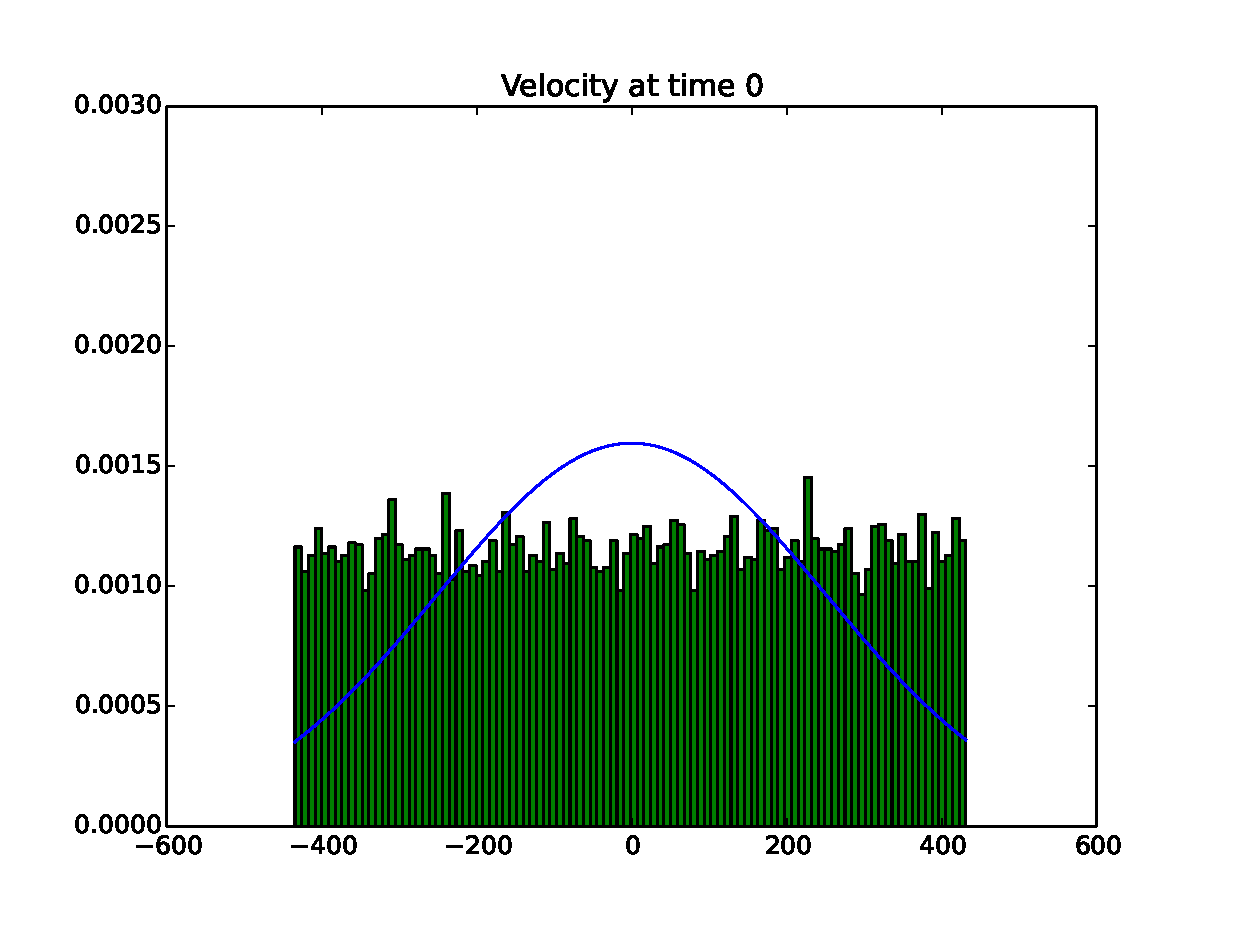
\includegraphics[width = 0.5 \textwidth]{Figures/velocityDistribution_0.eps}
			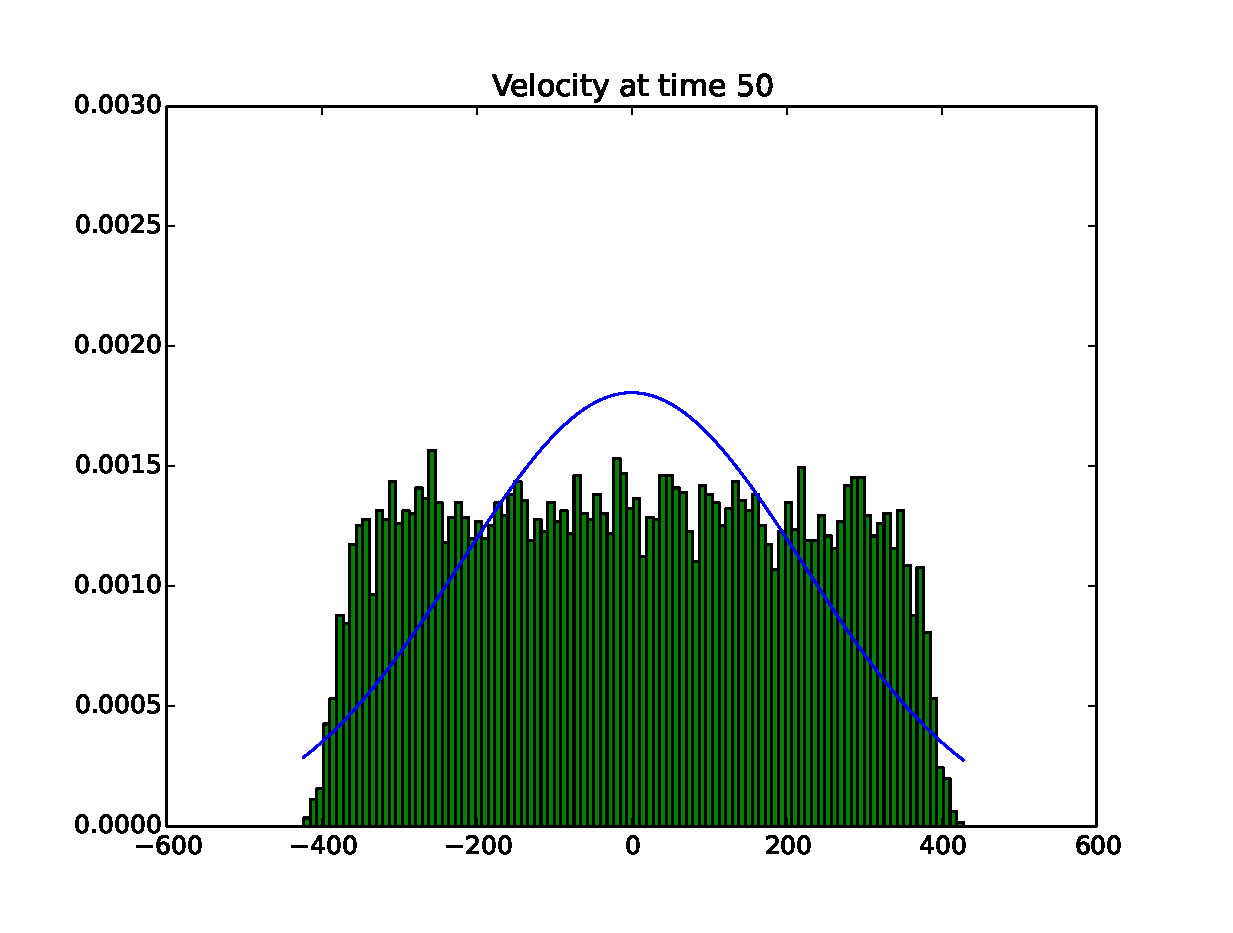
\includegraphics[width = 0.5 \textwidth]{Figures/velocityDistribution_50.eps}
			\end{subfigure}
			\begin{subfigure}{1\textwidth}
			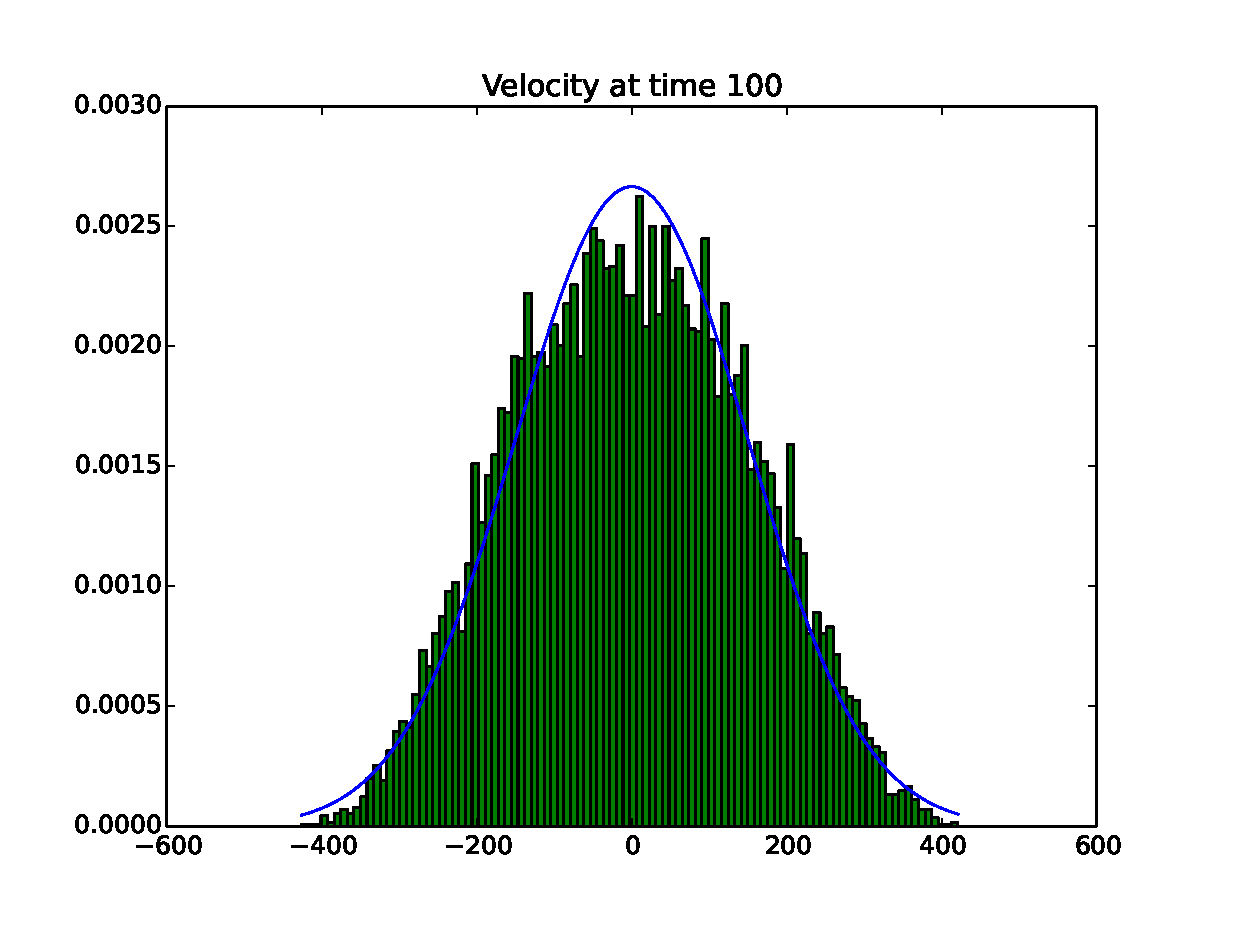
\includegraphics[width = 0.5 \textwidth]{Figures/velocityDistribution_100.eps}
			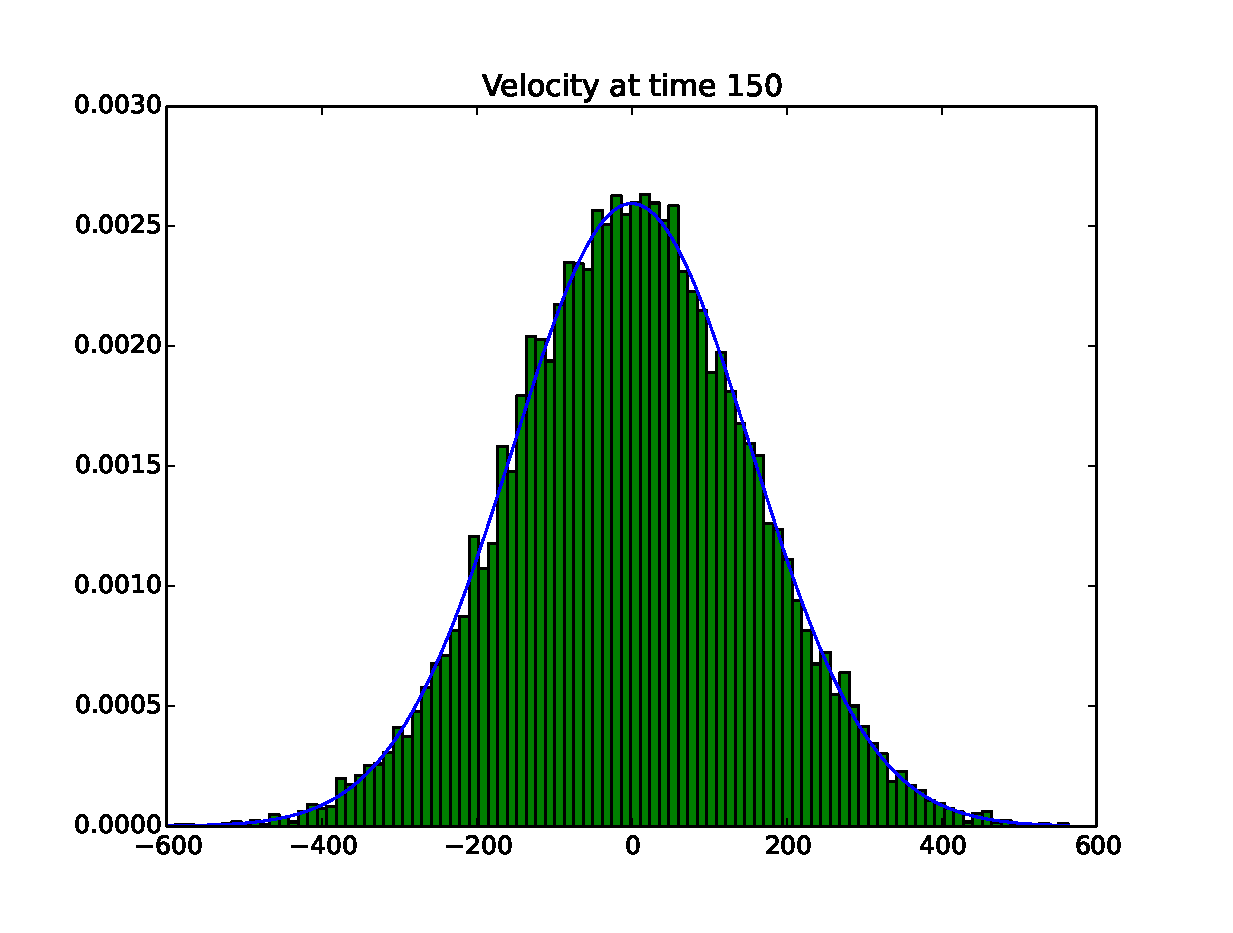
\includegraphics[width = 0.5 \textwidth]{Figures/velocityDistribution_150.eps}
			\end{subfigure}
			\caption{Four figures of the distribution of velocities in the x-direction first given an uniform distribution developing into a gaussian distribution, the line is the best gaussian fit.}
		\end{figure}



	\subsection{Task o: Radial distribution function}
		% \begin{figure}
		% 	\includegraphics{Figures/radialDist.eps}
		% \end{figure}

		Not completely done yet, need to divide radial distrbution function by area of shells and stuff, waiting with it for a while.



	\subsection{Task g: Implementing a thermostat}
		After initializing the system, it will after while stabilize with a different temperature than it was initialized in. So we will need to implement a thermostat and let that run for a while to get the system to maintain that temperature that we want to measure statistical properties at. In this project we will implement a Berendsen thermostat, that works by first calculating a scalar value ,\(\gamma\), for how much the temperature of the system is different from the wanted temperature, see equation \eqref{eq:berentsen}, where \(\gamma\) is the adjustment scalar, \( \Delta t \) is the timestep, \( T_Bath \text{ and } T\) is the measured and wanted temperatures, \(\tau\) is a relaxation factor. 

		\begin{align}
			\gamma &= \sqrt{ 1 - \frac{\Delta t}{\tau} \left( \frac{T_{Bath}}{T} - 1 \right) } \label{eq:berentsen}
		\end{align}

		Then all of the individual atoms velocities are multiplied with the factor \( \gamma\) and the temperature is increased, or decreases, to get closer to the wanted temperature.



\appendix
	\section{Unit scheme}

	We want to use a unit system so all the numbers are computed on a unity scale, this ensures that there will be no overflow and it is easy to check that the number are approximately correct.


		The program uses a more natural set of units which let's Boltzmann's constant be 1.

		\begin{align}
			1 \text{ mass unit } &=   39.948 \text{ a.m.u } =  39.948\times 1.661\cross 10^{-27} \text{ kg}
			\\
			1 \text{ length unit } &= 3.405 \text{ \AA} = 3.405\cross 10^{-10} \text{ m}
			\\
			1 \text{ energy unit } &= 1.651 \cross 10^{-21} \text{ J}
			\\
			1 \text{ temperature unit } &= 119.735 \text{ K}
		\end{align}


	All the other units are then expressed in term of these units.

	Boltzmann constant translates between temperature and energy, in SI-units it is \( k_B = 1.381 \cross 10^{-23} \text{ J K}^{-1}\), which in the previously defined units becomes
	\begin{align}
	k_B &= 1.381 \cross 10^{-23}  \left(\text{ J K}^{-1}\right)  \left(\frac{\text{energy unit}}{1.651 \cross 10^{-21} \text{ J}}\right)
	\left( \frac{119.735 \text{ K}}{\text{temperature unit}} \right)
	\\
	k_B &= 1 \; \frac{\text{energy unit}}{\text{temperature unit}}
	\end{align}




























\bibliography{mybib}{}
\bibliographystyle{plain}
		
\end{document}
